\chapter{Projektin lähtökohdat}
\label{ch:projektin-lähtökohdat}
Ennen tämän työn aloittamista yrityksessä oli jo kehitetty ensimmäinen versio ohjelmasta, joka kykeni tilaamaan viestejä IED-laitteelta. Prosessoimaan viestit ja tallentamaan ne relaatiotietokantaan myöhempää käyttöä varten. Tässä ohjelmistossa oli havaittuja ongelmia ja se ei myöskään tukenut kaikkia IEC 61850 -standardin viesteihin liittyviä ominaisuuksia. Tämän ohjelmiston toimintaperiaate ja siinä olleet ongelmat toimivat pohjana uuden version suunnittelulle ja toteutukselle. Tarkoituksena oli poistaa havaitut ongelmakohdat ja miettiä olisiko jokin muu arkkitehtuuri parempi kyseiseen toteutukseen. Ensimmäistä toteutusta ohjelmasta voisi nimittää ensimmäiseksi protoversioksi tai demovaiheeksi (engl. proof of consept), jonka pohjalta tultiin tekemään toimiva lopullinen versio. Tekstissä eteenpäin sanalla demoversio viitataan tähän ohjelmistoon.

Tässä osiossa pohjustetaan työn alkua lukijalle ja mistä lähdettiin liikkeelle. Mitä ongelmia demovaiheen toteutuksessa oli ja niiden analyysi. Demovaiheen ohjelmasta käsitellään sen arkkitehtuuria, mitkä olivat sen komponentit ja niiden toiminnallisuus. Tässä käsitellyt ongelmat toimivat pohjana uuden version suunnittelulle ja auttavat tekemään siihen liittyviä ratkaisuja.


\section{Demoversio ja sen toiminta}
\label{ch:demoversio-ja-sen-toiminta}
Demoversio oli ohjelmoitu Ruby-ohjelmointikielellä. Ohjelman arkkitehtuuri oli todella yksinkertainen. Kuvassa \ref{fig:demo-architecture} on esitetty demoversion arkkitehtuuri korkealla tasolla.

\begin{figure}
	\includegraphics[width=1\textwidth]{pictures/demo-architecture.png}
	\caption{Rubylla toteutetun demoversion arkkitehtuuri ja tiedonsiirto.}
	\label{fig:demo-architecture}
\end{figure}

Yksi ajettu demoversion prosessi pystyi tilaamaan yhden IED-laitteen kaikki RCB-luokkien instanssit. Tiedon instanssien olemassaolosta ohjelma pystyi lukemaan relaatiotietokannasta. Prosessoimaan viestit ja tallentamaan ne relaatiotietokantaan myöhempää käyttöä varten. Ruby-ohjelmistossa tärkeässä osassa oli libIEC61850-kirjasto\footnote{\url{http://libiec61850.com}}. libIEC61850-kirjasto on avoimen lähdekoodin C-kielellä toteutettu kirjasto, joka abstrahoi IEC 61850 -standardin matalan tason määrittämiä palvelukutsuja ja datarakenteita helpokäyttöiseksi rajapinnaksi. Kirjasto tarjosi toiminnallisuuden IED-laitteella olevan serveriohjelmiston, sekä IED-laittetta käyttävän asiakaohjelmiston toteuttamiseen. IED-laitteen serverille kirjasto tarjosi funktioita ja rakenteita IEC 61850 määrittämien luokkien ja hierarkian rakentamiseen ja käsittelyyn. IED-laitteen asiakasohjelmalle kirjasto tarjosi funktioita ja rakenteita standardin määrittämiin palveluihin, kuten arvojen lukuun ja asettamiseen, datajoukkojen käyttöön ja viestien tilaamiseen. Tätä samaa kirjastoa käytettiin myös tämän työn toteutetussa ohjelmistossa. Koska demoversiossa ja tämän työn toteutuksessa keskitytään vain asiakasohjelmiston tekemiseen, käytetään kirjastosta vain sen asiakasohjelman toteutuksen ominaisuuksia.

Kirjasto oli rakennettu käyttämään MMS-protokollaa tiedonsiirrossa IED-laitteen ja sen asiakasohjelman välillä, kuten IEC 61850 -standardin osassa 8-1 määritetään. Kuvassa \ref{fig:libiec61850-layer-architecture} on esitetty kirjaston kerrosarkkitehtuuri asiakasohjelmalle. Kirjastoon oli toteutettu laiteabstraktiokerros (engl. hardware abstraction layer, lyhennetään HAL). HAL:in avulla kirjasto voi toimia monella eri laitealustalla, ja käyttäjä voi tarvittaessa lisätä oman HAL-implementaation. Demoversiota ajettiin Linux-käyttöjärjestelmällä, joten kirjastosta käytettiin olemassa olevaa Linux HAL toteutusta. Kuvassa \ref{fig:libiec61850-layer-architecture} on punaisella merkitty laatikot, jotka kirjaston käyttäjä voi tarjota, keltaisella kirjaston uudelleenkäytettävät MMS-protokollan osuudet ja sinisellä IEC 61850 -standardin toteuttavat osuudet. Kuvaan on merkitty vihreällä demoversioon toteutetut osuudet, eli Ruby-kielelle liitos C-kieleen ja tämän päälle Rubylla ohjelmoitu demo.

\begin{figure}
	\includegraphics[width=1\textwidth]{pictures/libiec61850-layer-architecture.png}
	\caption{libIEC61850-kirjaston kerrosarkkitehruurin komponentit, vihreällä Ruby toteutukseen lisätyt osat (pohjautuu kuvaan \cite{libIEC61850-api-overview}).}
	\label{fig:libiec61850-layer-architecture}
\end{figure}

Ruby-koodista C-kielen funktioiden kutsuminen ei ole suoraan mahdollista, vaan kielten väliin täytyy toteuttaa liitos. Demoversiossa liitos oli tehty käyttäen Rubylle saatavaa ruby-ffi -kirjastoa\footnote{\url{https://github.com/ffi/ffi}} (engl. Foreign Function Interface, lyhennetään FFI). Liitoksen avulla Ruby voi kutsua C-kielen funktioita ja käyttää sen struktuureita ja muuttujia. Demossa kirjasto hoiti matalan tason IEC 61850 asiat, ja Ruby-koodi keskittyi liitoksen avulla korkean tason viestin parsintaan ja tallennukseen tietokantaan.


\section{Ongelmakohdat ja analysointi}
\label{ch:ongelmakohdat-ja-analysointi}
Demoversiossa ohjelma oli toteutettu Ruby on Rails kehyksen päällä ajettavaksi. Ruby on Rails kehys on tarkoitettu web-sovellusten toteuttamiseen Ruby kielellä. Se tarjoaa Active Record nimisen ORM-kerroksen (engl. Object-relational Mapping) tietokannan käsittelyn helpottamiseen. ORM-kerros abstrahoi relaatiotietokannan käyttämisen oliopohjaiseksi ja kyselyitä tietokantaan voi suoraan tehdä Ruby-kielellä. Demoversio käytti Railsin Active Record ORM-kerrosta tietokannan käyttämiseen. Eli ennen ohjelman ajamista ohjelmaan täytyi ladata Railsin ajoympäristö muistiin, joka aiheutti sen että yksinkertaisen ohjelman täyti varata iso määrä muistia ennen suoritusta. Linuxin htop-ohjelmalla katsottuna, prosessi varasi noin 150 Mt muistia ajoa varten.

Ohjelma luki tietokannasta IED-laitteen, sekä sen kaikki RCB-instanssien tiedot. Tietojen avulla ohjelma tiesi mikä IED-laitteen IP-osoite on ja mitkä olivat RCB-instanssien referenssit. Ohjelmaan pystyi syöttämään eri tietoja ainoastaan tietokannan kautta ennen ajoa. Tämän jälkeen ohjelman toiminta, jokaisen RCB-instanssin viestien tilaukseen ja prosessointiin on esitetty sekvenssikaaviossa kuvassa \ref{fig:sequence-diagram-report-subscription}. Kuvassa ohjelman kaksi eri silmukkaa on esitetty kahdella eri loop-laatikolla. Sekvenssikaaviossa osallisena ovat tietokanta, Ruby-ohjelma, libIEC61850-kirjasto, libIEC61850-kirjaston natiivisäie ja IED-laiteen palvelinohjelma. Rubyn ja libIEC61850-kirjaston liitos oli tehty ruby-ffi -kirjastolla ja kirjaston natiivisäie on vastuussa yhteyden ylläpidosta ja datan siirtämisestä. Sekvenssikaavioon on merkitty paksulla suorituksessa olevat palkit minäkin ajan hetkenä, esimerkiksi IED-laitteen palvelinohjelmisto on koko ajan ajossa.

\begin{figure}
	\includegraphics[width=1\textwidth]{pictures/sequence-diagram-report-subscription.png}
	\caption{Sekvenssikaavio kaikkien RCB-instanssien tilaukseen ja niiden viestien tallentamiseen yhdeltä IED-laitteelta Ruby-ohjelmalla.}
	\label{fig:sequence-diagram-report-subscription}
\end{figure}

Tietokannasta luettujen tietojen jälkeen ohjelma muodostaa yhteyten IED-laitteelle, ensin tekemällä instanssin \texttt{IedConnection} struktuurista funktiolla \texttt{IedConnection\_create()}. Tämän jälkeen struktuuri annetaan \texttt{IedConnection\_connect()} funktiolle, joka avaa yhteyden IED-laitteelle ja palaa vasta kun vastaus saapuu. Tässä vaiheessa libIEC61850-kirjasto käynnistää erillisen natiivisäikeen yhteyden viestien vastaanottoon. Tämä tapahtuu kirjaston lähdekoodissa src/mms/iso\_client/iso\_client\_connection.c funktiossa \texttt{IsoClientConnection\_associate()} riveillä 429--434 \cite{libIEC61850-repo}. Tätä säiettä kirjasto käyttää tulevien viestien vastaanottoon ja lähettämiseen. Yhteyden avauksen jälkeen jokainen RCB-instanssi tilataan lukemalla ensin sen arvot IED-laitteelta funktiolla \texttt{IedConnection\_getRCBValues()}. Funktiokutsu nukkuu ja palaa vasta kunnes erillinen säie ilmoittaa että vastaus on saapunut, tai yhteyden aika ylittyy. Kirjaston funktio, joka tämän hoitaa on \texttt{sendRequestAndWaitForResponse()} ja on määritetty src/mms/iso\_mms/client/mms\_client\_connection.c riveillä 345--418 \cite{libIEC61850-repo}. RCB-arvot luettuaan, kirjasto palauttaa struktuurin \texttt{ClientReportControlBlock}, joka sisältää luetut tiedot RCB-instanssista. Samaa struktuuria käytetään arvojen muuttamiseen ja niiden takaisin kirjoittamiseen IED-laitteelle. Ennen muunneltujen RCB-arvojen takaisin kirjoittamista ja viestien tilaamista, täytyy kirjastolle asettaa takaisinkutsufunktio, jota kirjastoo kutsuu aina kun tilattu viesti saapuu IED-laitteelta. Takaisinkutsufunktio asetetaan \texttt{IedConnection\_installReportHandler()}, joka ottaa parametrikseen funktiopointterin ja vaihtoehtoisen parametripointterin. Asetuksen ajaksi kirjasto lukitsee \texttt{reportHandlerMutex}. Jos lukituksen aikana saapuu viesti, joutuu erillinen säie nukkumaan ja odottamaan lukituksen vapautusta, kohdat 33--36. Tämän jälkeen arvot kirjoitetaan takaisin IED-laitteelle funktiolla \texttt{IedConnection\_setRCBValues()}. Tämä funktio myös palaa vasta kunnes IED vastaa, tai yhteyden aika ylittyy, kuten aikaisemmin. Heti arvojen kirjoitusten jälkeen IED aloittaa lähettämään viestejä tilaajalle. Eli samalla kun muita RCB-instansseja tilataan, jo tilatut RCB-instanssit lähettävät jo viestejä ja aiheuttavat takaisinkutsufunktion suorittamisen. Kun kaikki RCB-instanssit on tilattu, ohjelma jää viimeiseen silmukkaan odottamaan ja prosessoimaan viestejä. Kun viesti saapuu, säie kutsuu ensin sisäisesti \texttt{mmsIsoCallback()} funktiota, joka kutsuu muita kirjaston sisäisiä funktioita ja lopuksi asetettua takaisinkutsufunktiota. Takaisinkutsufunktio on liitetty Ruby funktioon ja funktio tallentaa raportin tiedot tietokantaan. Ruby-funktion suorituksen ajaksi kirjasto lukitsee \texttt{reportHandlerMutex}, ja vapautetaan kunnes Ruby-funktion suoritus palaa. Tätä jatkuu niin kauan kunnes ohjelmalle lähetetään jokin signaali, joka lopettaa sen suorituksen. \cite{Kozlovski2017, Storimer2013}

Demossa isoimpana ongelmana oli sen huono suorituskyky ja toiminnan epävarmuus RCB-instanssien määrän ollessa enemmän kuin muutama. RCB-instanssien määrän ollessa liian suuri, ohjelma saattoi epäonnistui joidenkin tilaamisessa, koska yhteys aikakatkaisi arvojen kirjoituksessa tai luvussa. Lisäksi, jotta kaikki RCB-instanssit saatiin edes tilattua, saattoi ohjelmalta kestää siinä noin puoli minuuttia esimerkiksi tilata 13 RCB-instanssia.

Huonoon suorituskykyyn oli syynä muutama asiaa. Yksi niistä oli Ruby-kielen huonompi suorituskyky verrattuna natiivisti käännettyyn C-kieleen. Ruby on tulkattava kieli kuten esimerkiksi Python, joka tulkataan rivi kerrallaan ja suoritetaan. Lähdekoodia ei käännetä kokonaan ensin konekäskyiksi erillisellä kääntäjällä, kuten C-kielessä. Valmiiksi käännetty lähdekoodi tarvitsee vain ajaa, kun taas tulkattavassa kielessä rivi täytyy ensin tulkata ja sitten ajaa. Rubyssa käytettiin sen oletustulkkia MRI/YARV (engl. Matz's Ruby Interpreter, lyhennetään MRI tai Yet another Ruby VM, lyhennetään YARV). Ruby versiosta 1.9 eteenpäin käyttää YARV tulkkia. Toinen syy oli Ruby-kielen oletustulkissa oleva globaali tulkkilukitus (engl. global interpreter lock, lyhennetään GIL, tai global virtual machine lock, lyhennetään GVL). GIL pakottaa Ruby-ohjelman ajoon vain yhdellä CPU:lla ja vain yksi säie vuorossa kerrallaan ja on riippumaton käyttöjärjestelmän kernelin vuorottajasta \cite[s.~131--133]{Odaira2014}. Kuvassa \ref{fig:ruby-gil} on esitetty kuinka Ruby-tulkki vuorottaa kahta ajossa olevaa säiettä. Kuvassa Demon Ruby koodi kutsuu \texttt{IedConnection\_setRCBValues()} funktiota, ajo jää kesken ja tapahtuu vaihto, koska viesti saapui. Takaisinkutsufunktio suoritetaan ja suoritus palaa takaisin aikaisempaan funktion suoritukseen. Tässä vaiheessa jos vaihto on huonolla hetkellä vaihto kesti liian kauan, tulee yhteyden aikakatkaisu ja RCB-instanssi jää tilaamatta. Huonoon suorituskykyyn mahdollisesti vaikutti myös lukitus \texttt{reportHandlerMutex}, jota kirjastossa käytetään kun takaisinkutsufunktio asetetaan ja takaisinkutsufunktio suoritetaan. Lukitus aiheuttaa säikeen nukkumisen niin kauan kunnes lukitus vapautuu. Tässä tapauksessa, jos viestin prosessointi kestää kauan (kuvassa \ref{fig:sequence-diagram-report-subscription} kohdat 33--36). Ja vielä muita RCB-instansseja tilataan silmukassa (kohdat 12--26). Joutuu säie odottamaan lukituksen vapautusta kun takaisinkutsufunktioita asetetaan (kohdat 19--20). Ratkaisuna tähän olisi pitää takaisinkutsufunktio mahdollisimman lyhyenä suoritusajan suhteen.

\begin{figure}
	\includegraphics[width=1\textwidth]{pictures/ruby-gil.png}
	\caption{Ruby-tulkin globaalin lukituksen toiminta, joka vuorottaa ajossa olevia säikeitä.}
	\label{fig:ruby-gil}
\end{figure}

Tämän lisäksi demototeutuksessa oli muistivuoto, joka söi muistia ja sitä ei ikinä vapautettu. Muistivuoto johtui todennäköisesti jostakin ohjelmointivirheestä ruby-ffi -kirjaston liitoksen kanssa. Kun liitos Rubysta tehdään C-kieleen, täytyy ohjelmoidan miettiä roskien keruuta tarkasti. Tätä ei normaalisti tarvitse miettiä ollenkaan Rubyssä, koska tulkki implementoi automaattisen roskien keruun. Muistivuoto havaittiin kun ohjelman jättää ajoon pitemmäksi aikaa, on ohjelma varannut melkein kaiken käyttöjärjestelmän muistista itselleen. Lisäki jos ohjelmaa ajaa ja tarkkailee Linuxin htop-ohjelmalla, voi MEM\%-sarakkeesta huomata prosentuaalisen osuuden kasvavan koko käyttöjärjestelmän muistista. Tulevaisuutta ajatellen lopullinen tiedon tallennuspaikka ei ole muiden tietoa tarvitsevien ohjelmien kannalta järkevä. Näiden ohjelmien pitäisi koko ajan olla kyselemässä uusinta tietoa tietokannasta erikseen. Tämä kuormittaisi turhaan tietokantaa ja varsinkin jos tietoa tarvitsevia ohjelmia on useita.